\section{Persistence Properties}
\label{sec-pp}

In this section, we study the {\em persistence properties} of modern file
systems. These properties determine which possible post-crash file system
states are possible for a given file system; as we will see, different file
systems provide subtly different guarantees, making the challenge of building
correct application protocols atop such systems more vexing.

We begin with an example, and then describe a simple tool we've built, known
as the {\em Block Order Breaker (\fstoolname)}, that explores possible on-disk states
by reordering the I/O block stream and examining possible resulting states.
\fstoolname\ is not a complete tool, but can be used to find persistence properties
that do {\em not} hold for a file system implementation. We then discuss our
findings for six widely-used Linux file systems (ext2~\cite{CardEtAl94-Ext2},
ext3~\cite{Tweedie98-JournalingExt2, Tweedie00-Ext3Talk},
ext4~\cite{TsoTweedie02-Ext23}, btrfs~\cite{Mason07-btrfs},
xfs~\cite{SweeneyEtAl96-XFS}, and reiserfs~\cite{Reiser04-ReiserFS}).

Application-level crash consistency depends strongly upon these persistence
properties, yet there are currently no standards.  We believe that defining
and studying persistence properties is the first step towards standardizing
them across file systems. 

\subsection{An Example}
\label{sec-ppexample}

All application update protocols boil down to a sequence of I/O-related system
calls which modify on-disk state. Two broad properties of system calls affect
how they are persisted. The first is \textit{atomicity}: does the update from
the call happen all at once, or are there possible intermediate states that
might arise due to an untimely crash?  The second is \textit{ordering}: can
this system call be persisted \textit{after} a later system call? We now
explain these properties with an example.

\begin{figure}[!t]
\centering
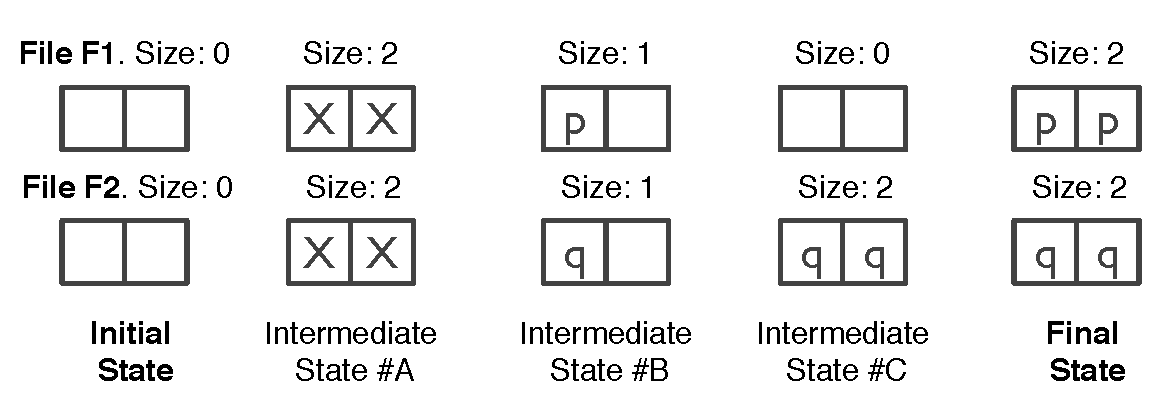
\includegraphics[scale=0.4]{figs/crashstates.eps}
\mycaption{fig-crashstates}{Crash States}{\footnotesize 
The figure shows the initial, final, and some of the intermediate crash states
possible for the workload described in Section~\ref{sec-ppexample} . X
represents garbage data in the files. Intermediate states \#A and \#B represent
different kinds of atomicity violations, while intermediate state \#C
represents an ordering violation.
}
\end{figure}




\noindent We consider the following pseudo-code snippet:
\vspace{-0.05in}
\begin{Verbatim}[fontsize=\footnotesize, baselinestretch=0.1, commandchars=\\\{\},
framesep=0pt]
  \vspace{1in}
  write(f1, "pp");
  write(f2, "qq");
\end{Verbatim}
\vspace{-0.1in}
In this example, the application first appends the string \smalltt{pp} to file
descriptor \smalltt{f1} and then appends the string \smalltt{qq} to file
descriptor \smalltt{f2}. Note that we will sometimes refer to such a
\smalltt{write()} as an \smalltt{append()} for simplicity.

Figure~\ref{fig-crashstates} shows the possible crash states that can result.
If the append is not {\em atomic}, for example, it would be possible for the
{\em size} of the file to be updated without the new data reflected to disk; in
this case, the files could contain garbage, as shown in State A in the diagram.
We refer to this as \textit{size-atomicity}. A lack of atomicity could also be
realized with only part of a write reaching disk, as shown in State B. We refer
to this as \textit{content-atomicity}.

If the file system persists the calls out of order, another outcome is possible (State
C). In this case, the second write reaches the disk first, and as a result
only the second file is updated. Various combinations of these states are also
possible.

As we will see when we study application update protocols, modern applications
expect different atomicity and ordering properties from underlying file
systems. We now study such properties in detail.

\subsection{The Block Order Breaker (BOB)}
\label{sec-fs-properties}

We study the persistence properties of six Linux file systems: ext2, ext3,
ext4, btrfs, xfs, and reiserfs. A large number of applications have been
written targeting these file systems. Many of these file systems also provide
multiple configurations that make different trade-offs between performance and
consistency: for instance, the data journaling mode of ext3 provides the
highest level of consistency, but often results in poor
performance~\cite{PrabhakaranEtAl05-Usenix}.  Between file systems and their
various configurations, it is challenging to know or reason about which
persistence properties are provided.  For this reason, we examine different
configurations of the file systems we study (a total of 16).

To study persistence properties, we built a tool, known as the
\textit{Block Order Breaker} (\fstoolname), to empirically find cases where
various persistence properties do {\em not} hold for a given file system.
\fstoolname\ first runs a workload designed to stress the persistence property
tested (e.g., a number of writes of a specific size to test overwrite
atomicity).  \fstoolname\ collects the block I/O generated by the
workload. \fstoolname\ then re-orders the collected blocks and selectively
writes some of them to the initial disk state to generate a new legal disk state. In
this manner, \fstoolname\ generates a number of unique disk images
corresponding to possible on-disk states after a system crash.
\fstoolname\ then checks whether the persistence property holds (e.g., if the
writes were atomic) on each disk image. If \fstoolname\ finds even a single
disk image where the checker fails, then we know that the property does not
hold on the file system. Proving the converse (a property holds in all
situations) is not possible using \fstoolname.

Note that different system calls (e.g., \smalltt{write()}, \smalltt{writev()})
lead to the same file system output. We group such calls together into a
generic file system update we term an \textit{operation}. We have found that
grouping all operations into three major categories is sufficient for our
purposes here: file overwrite, file append, and directory operations
(including rename, link, unlink, mkdir, etc.).  

\begin{table}[!t]
\begin{center}
\setlength{\tmpa}{\tabcolsep}
\setlength{\tabcolsep}{0.7pt}
{\footnotesize
\begin{tabular}{l|l*{15}c}
%{\multirow{3}{*}{\bf PCP}} & {\multicolumn{10}{c}{\bf Filesystem}} \\ 
%\cline{2-8}
\textbf{Persistence Property} & \multicolumn{15}{c}{\bf File system}  \\[2ex]
\hline
%\hline \\ [-2ex]
& \rotatebox{90}{ext2}
& \rotatebox{90}{ext2-sync}
& \rotatebox{90}{ext3-writeback}
& \rotatebox{90}{ext3-ordered}
& \rotatebox{90}{ext3-datajournal}
& \rotatebox{90}{ext4-writeback}
& \rotatebox{90}{ext4-ordered}
& \rotatebox{90}{ext4-nodelalloc}
& \rotatebox{90}{ext4-datajournal}
& \rotatebox{90}{btrfs}
& \rotatebox{90}{xfs}
& \rotatebox{90}{xfs-wsync}
& \rotatebox{90}{reiserfs-nolog}
& \rotatebox{90}{reiserfs-writeback}
& \rotatebox{90}{reiserfs-ordered}
& \rotatebox{90}{reiserfs-datajournal~}
\\ 
\hline
% Atomicity properties
\textbf{Atomicity} & & & & & & & & & & & & & & & \\
\hline
Single sector overwrite & & & & & & & & & & & & & & & \\
\hline
Single sector append  & \fwrong & &  \fwrong & & &  \fwrong & & & & & & & &  \fwrong & & \\
\hline
Single block overwrite & \fwrong &  \fwrong &  \fwrong &  \fwrong & &  \fwrong &  \fwrong &  \fwrong & &  &  \fwrong &  \fwrong &  \fwrong &  \fwrong &  \fwrong & \\
\hline
Single block append & \fwrong &  \fwrong &  \fwrong & & &  \fwrong & & & & & & &  \fwrong &  \fwrong & & \\
\hline
Multi-block append/writes~ & \fwrong &  \fwrong &  \fwrong &  \fwrong &  \fwrong &  \fwrong &  \fwrong &  \fwrong &  \fwrong &  \fwrong &  \fwrong &  \fwrong &  \fwrong &  \fwrong &  \fwrong &  \fwrong \\
\hline
Multi-block prefix append~ &  \fwrong & \fwrong &  \fwrong & & &  \fwrong & & &
& & & & \fwrong &  \fwrong & & \\
\hline
Directory op & \fwrong & \fwrong & & & & & & & &  & & & \fwrong & & & \\
\hline
% Ordering properties
\textbf{Ordering} & & & & & & & & & & & & & & & \\
\hline
Overwrite $\to$ Any op~ &  \fwrong &  &  \fwrong &  \fwrong & &  \fwrong &  \fwrong &  \fwrong & & &  \fwrong &  \fwrong &  \fwrong &  \fwrong &  \fwrong & \\
\hline
[Append, rename]$\to$ Any op~  &  \fwrong & &  \fwrong & & &  \fwrong & & & & & & & \fwrong &  \fwrong & & \\
\hline
\verysmalltt{O\_TRUNC} Append $\to$ Any op &  \fwrong & &  \fwrong & & & \fwrong & & & & & & & \fwrong &  \fwrong & & \\
\hline
Append $\to$ Append (same file)  &  \fwrong & &  \fwrong & & &  \fwrong & & & & & & & \fwrong &  \fwrong & & \\
\hline
Append $\to$ Any op &  \fwrong & &  \fwrong & & &  \fwrong &  \fwrong & & & \fwrong &  \fwrong & & \fwrong &  \fwrong & & \\
\hline
Dir op $\to$ Any op &  \fwrong & & & & & & & & &  \fwrong & & & \fwrong & & & \\
\end{tabular}
}
\end{center}
\vspace{-0.1in}
\mycaption{tbl-ppresults}{Persistence Properties}{\footnotesize
The table shows atomicity and ordering persistence properties that we
empirically determined for different configurations of file systems. X $\to$ Y
is persisted before Y. [X,Y] $\to$ Z indicates that Y follows
X in program order, and both become durable before Z. A \fwrong\ indicates that
we have a reproducible test case where the property fails in that file system.
} 
\setlength{\tabcolsep}{\tmpa}
\end{table}


Table~\ref{tbl-ppresults} lists the results of our study. The table shows, for
each file system (and specific configuration) whether a particular persistence
property has been found to {\em not} hold; such cases are marked with an
$\times$. 

The size of an overwrite or append affects its atomicity. Hence, we show results
for single sector, single block, and multi-block overwrite and append
operations. As for ordering, we show whether given properties hold
assuming different orderings of overwrite, append, and directory
operations; the append operation has some interesting special cases
relating to delayed allocation (as found in Linux ext4) -- we show these
separately. 

\subsubsection{Atomicity}

We observe that all tested file systems provide atomic single sector
overwrites: in some cases (e.g., ext2), this is because the underlying disk
 provides atomic sector writes. Note that if such file systems are run on
top of new technologies such as PCM that provide atomicity at byte
granularity~\cite{condit2009better}, single-sector overwrites will not be
atomic.

Providing atomic appends requires the update of two locations (file inode,
data block) atomically. Doing so requires file-system machinery, and is not
provided by ext2 or writeback configurations of ext3, ext4, and reiserfs.

Overwriting an entire block atomically requires data journaling or
copy-on-write techniques; atomically appending an entire block can be done using
ordered mode journaling, since the file system only needs to ensure the entire
block is persisted before adding a pointer to it.

Current file systems do not provide atomic multi-block appends -- appends can
be broken down into multiple operations. However, most file systems do
guarantee that some prefix of the data written (e.g., the first 10 blocks of a
larger append) will be appended atomically.

Directory operations such as \smalltt{rename()} and \smalltt{link()} are atomic
on all file systems that use techniques like journaling or copy-on-write for
consistency. 

\subsubsection{Ordering}

We observe that ext3, ext4, and reiserfs in data journaling mode, and ext2 in
sync mode, persist all tested operations in order. Note that these modes often
result in poor performance on many workloads~\cite{PrabhakaranEtAl05-Usenix}.

The append operation has interesting special cases. On file systems with
delayed allocation, it may be persisted after other operations. A special
exception to this rule is when a file is appended to, and then renamed. Since
this idiom is commonly used to atomically update
files~\cite{URLmassivefsthread}, many file systems recognize it and allocate
blocks immediately. A similar special case is appending to files that have
been opened with \smalltt{O\_TRUNC}. Even with delayed allocation, successive
appends to the same file are persisted in order. ext2 and btrfs freely
re-order directory operations (especially operations on different
directories~\cite{btrfs-mason}) to increase performance.

\subsection{Summary}

From Table~\ref{tbl-ppresults}, we observe that persistence properties vary
\textit{widely} among file systems, and even among different configurations of
the same file system. The order of persistence of system calls depends upon
small details like whether the calls are to the same file or whether the file was
renamed. From the viewpoint of an application developer, it is very risky to
assume that any particular property will be supported by all file systems. 
